\documentclass{standalone}
\usepackage{pgfplots}
\pgfplotsset{width=9cm, compat=1.5}
\begin{document}
	\begin{tikzpicture}
	\begin{axis}[
	xlabel=$\varepsilon_x$,
	ylabel=Magnetizaci\'on $(\mu_B)$]
	
	\addplot table [x=e, y=mag] {magn.dat};
	\node at (300,150) {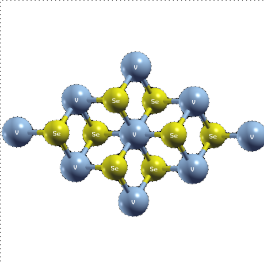
\includegraphics[scale=0.17]{est_0.0}};
	\node at (450,20) {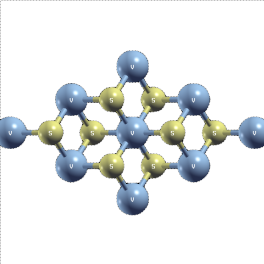
\includegraphics[scale=0.2]{est_0.03}};
	\node at (50,150) {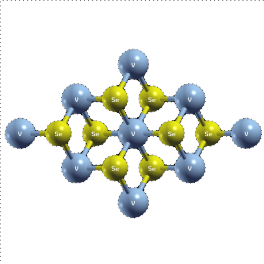
\includegraphics[scale=0.17]{est_-0.03}};
	\draw[->, color=black, very thick](50,175)--(10,190);
	\draw[->, color=black, very thick](520,10)--(590,2);
	\draw[->, color=black, very thick](300,175)--(300,190);
	\end{axis}
	
	\end{tikzpicture}
\end{document}
